\documentclass[12pt,a4paper]{article}
\usepackage{fontspec}
\setmainfont{Latin Modern Sans}
\usepackage{xcolor}
\definecolor{primary}{RGB}{0,103,149}
\definecolor{secondary}{RGB}{128,179,211}
\definecolor{highlight}{RGB}{242,120,75}
\usepackage{graphicx}
\usepackage[a4paper,margin=2.5cm]{geometry}
\usepackage{titlesec}
\usepackage{colortbl}


\titleformat{\section}
  {\color{primary}\Large\bfseries\sffamily}
  {\thesection}{1em}{}[\color{primary}\titlerule]
\titleformat{\subsection}
  {\color{primary}\large\bfseries\sffamily}
  {\thesubsection}{1em}{}
\titleformat{\subsubsection}
  {\color{secondary}\normalsize\bfseries\sffamily}
  {\thesubsubsection}{1em}{}

\usepackage{enumitem}
\setlist[itemize]{leftmargin=1.5em, label=\textcolor{primary}{\textbullet}, itemsep=0.5em, parsep=0.2em}
\setlist[enumerate]{leftmargin=1.5em, itemsep=0.5em, parsep=0.2em}

\usepackage{float}
\usepackage{tabularx}
\usepackage{booktabs} 
\renewcommand{\arraystretch}{1.4}
\setlength{\tabcolsep}{8pt}

\usepackage{hyperref}
\hypersetup{
    colorlinks=true,
    linkcolor=primary,
    urlcolor=primary,
    citecolor=primary
}

\usepackage[numbers,sort&compress]{natbib}

\usepackage{tcolorbox}
\tcbuselibrary{breakable, skins}

\newtcolorbox{summary}{
  enhanced,
  colback=secondary!20,
  colframe=primary,
  boxrule=1pt,
  fonttitle=\bfseries\sffamily,
  colbacktitle=primary,
  coltitle=white,
  attach boxed title to top left={yshift=-2mm, xshift=5mm},
  title=Executive Summary,
  breakable
}

\newtcolorbox{keyfinding}{
  enhanced,
  colback=highlight!15,
  colframe=highlight,
  boxrule=0.5pt,
  sharp corners,
  left=5pt,
  right=5pt,
  top=5pt,
  bottom=5pt,
  breakable
}

% Document starts
\begin{document}

% Improved title page
\begin{titlepage}
    \centering
    \vspace*{1cm}
    
    % Top rule
    \rule{\linewidth}{1pt}\vspace{0.5cm}
    
    % Title with better spacing and formatting
    {\Huge\bfseries\textcolor{primary}{Salesforce Application\\Security Audit}}\vspace{0.2cm}
    
    {\Large\textcolor{primary}{Case Study}}\vspace{0.5cm}
    
    % Bottom rule under title
    \rule{\linewidth}{1pt}\vspace{1.5cm}
    
    % Author information with improved spacing
    {\large\textit{Prepared by}}\vspace{0.5cm}
    
    {\Large\bfseries Kurudunje Deekshith Shetty}\vspace{0.3cm}
    
    {\large Security Analyst / Student}\vspace{2cm}
    
    % Image with frame and shadow effect
    \begingroup
    \setlength{\fboxsep}{0pt}
    \setlength{\fboxrule}{1pt}
    \fcolorbox{primary}{white}{%
        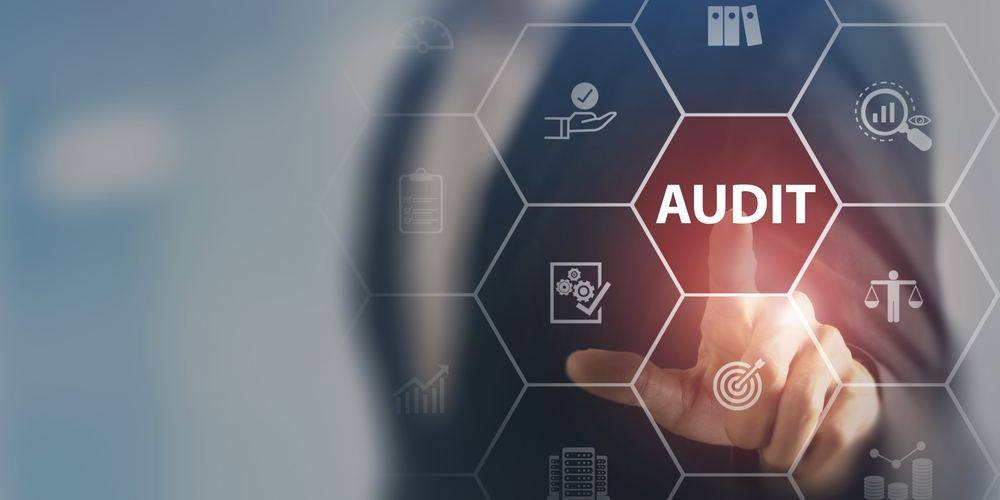
\includegraphics[width=0.8\textwidth]{audit.jpg}%
    }\vspace{1.5cm}
    \endgroup
    
    % Document information block
    \begin{tabularx}{\textwidth}{>{\raggedleft\arraybackslash}X>{\raggedright\arraybackslash}X}
    \textbf{Date:} & April 27, 2025 \\
    \textbf{Version:} & 1.0 \\
    \textbf{Status:} & Final Report \\
    \end{tabularx}\vspace{1cm}
    
\end{titlepage}

% Table of contents
\tableofcontents
\clearpage

% Executive summary before abstract
\begin{summary}
This study analyzes a recent cybersecurity incident where the threat actor "betway" compromised multiple Salesforce Cloud portals through stolen credentials. The key vulnerabilities exploited included weak authentication mechanisms, excessive user privileges, and inadequate monitoring systems. Our findings suggest implementing robust multi-factor authentication, enforcing least privilege principles, and enhancing monitoring capabilities as critical mitigation strategies. Organizations using Salesforce should prioritize these security controls to prevent similar breaches in the future.

\vspace{0.5em}
\textbf{Key Impact:} Stolen data from 6 organizations was offered for sale at prices ranging from \$5,000 to \$75,000, demonstrating the significant financial motivation behind these attacks and their potential business impact.
\end{summary}
\vspace{1cm}

\begin{abstract}
\textit{This case study examines a cyber campaign targeting Salesforce Cloud portals, as reported by ReliaQuest in their April 2025 report. The breach, attributed to stolen credentials, exposed vulnerabilities in authentication, access controls, and monitoring. Without direct Salesforce access, this study applies security audit procedures theoretically, drawing on online sources and best practices to identify weaknesses and propose mitigations. Key findings include weak authentication, over-privileged accounts, and inadequate monitoring, with recommendations for multi-factor authentication, least privilege, and enhanced monitoring. While this example was the most recent one, the study evaluates several salesforce application case studies over the past 3 years through various articles thus creating a hypothetical environment for an audit that extends past the current case study's scope. Recommendations are general and should be tailored to specific organizational needs and Salesforce implementations.}
\end{abstract}

\section{Introduction}
In April 2025, ReliaQuest reported a cybercriminal campaign targeting public-facing Salesforce Cloud portals, where a threat actor, ``betway,'' offered stolen data from six organizations for \$5,000 to \$75,000~\cite{reliaquest2025}. The breach resulted from compromised credentials, likely obtained through infostealer malware. Lacking direct access to Salesforce, this study hypothetically applies security audit procedures, leveraging online articles, industry reports, and best practices to analyze the incident and propose mitigation strategies.

\subsection{Background}
Salesforce is a leading customer relationship management (CRM) platform used by organizations worldwide to manage customer data, sales processes, and marketing campaigns. As cloud-based systems become increasingly important for business operations, they also become attractive targets for cybercriminals seeking valuable data.
\\\\

\subsection{Objectives}
This security audit aims to:
\begin{itemize}
    \item Identify security vulnerabilities in typical Salesforce implementations
    \item Analyze attack vectors used in recent breaches
    \item Develop pragmatic recommendations to enhance security posture
    \item Provide a framework for ongoing security monitoring
\end{itemize}

\subsection{Scope and Limitations}
This study is limited to theoretical analysis based on publicly available information and best practices, without direct access to affected Salesforce environments. The findings and recommendations represent hypothetical scenarios derived from industry standards and published security guidelines.

\section{Problem Statement}
The incident involved unauthorized access to Salesforce Cloud instances via stolen credentials, leading to significant data breaches. Public reports indicate that weak authentication mechanisms, insufficient monitoring of public-facing portals, and poor credential management enabled attackers to exploit Salesforce CRM systems, compromising sensitive customer data. This hypothetical audit assesses the security posture of a typical Salesforce environment, identifies potential weaknesses, and recommends controls based on online research and established audit methodologies.

\begin{keyfinding}
\textbf{Critical Security Issue:} The primary attack vector appears to be credential theft, with attackers using "infostealer" malware to obtain valid Salesforce login credentials. Once obtained, these credentials provided direct access to sensitive customer data with minimal technical barriers.
\end{keyfinding}

\section{Security Audit Methodology}
The audit methodology was designed to systematically evaluate the security controls of a typical Salesforce environment, drawing on standard practices and tools described in online sources~\cite{capstorm2023,foundhq2025,onilab2024,salesforce2025,sentinelone2024,sonar2025}.

\subsection{Pre-Audit Planning}
\subsubsection{Scope Definition}
The audit scope was defined to cover:
\begin{itemize}
    \item Authentication mechanisms and credential security
    \item User permissions and access controls
    \item Public-facing portal configurations
    \item Monitoring and incident response capabilities
    \item Custom code security
\end{itemize}

\subsubsection{Tools and Resources}
The following tools were considered for the hypothetical audit:
\begin{itemize}
    \item Salesforce Security Health Check
    \item OWASP ZAP for external portal vulnerability scanning
    \item Splunk for log analysis and correlation
    \item Checkmarx for static code analysis
    \item Burp Suite for session testing
\end{itemize}

\subsection{Audit Procedures}
The audit procedures were structured into six key areas:

\subsubsection{Access Control Review}
User profiles, roles, and sharing rules were evaluated for adherence to the principle of least privilege, using tools like Setup Audit Trail and Permission Set Analyzer to identify over-privileged accounts, as recommended by~\cite{onilab2024}.

\subsubsection{Authentication Review}
Multi-factor authentication (MFA) implementation, password policies, and session management were assessed, leveraging tools such as MFA Configuration Scanner and Burp Suite for session testing, following best practices for credential security~\cite{foundhq2025}.

\subsubsection{Vulnerability Scanning}
Dynamic and static application security testing (DAST and SAST) were proposed for portals and custom Apex code, using OWASP ZAP, Metasploit, and Checkmarx to detect vulnerabilities like XSS, as emphasized by~\cite{capstorm2023}.

\subsubsection{Log Analysis}
Login logs, API calls, and audit trails were analyzed for suspicious activity, with Splunk and Salesforce Event Monitoring as hypothetical tools to review monitoring configurations~\cite{sonar2025}.

\subsubsection{Incident Response Review}
Incident detection, containment, and recovery plans were evaluated, using Salesforce Security Center and Jira for tracking and workflow automation, in line with industry standards~\cite{onilab2024}.

\subsubsection{User Awareness Assessment}
Training programs, phishing awareness, and security culture were evaluated to assess the human element of security controls.

\begin{table}[H]
\caption{Criticality Index of Audit Procedures}
\label{tab:procedures}
\centering
\begin{tabularx}{\textwidth}{|X|l|c|}
\hline
\rowcolor{primary!20}
\textbf{Procedure} & \textbf{Scope} & \textbf{Criticality} \\
\hline
Pre-Audit Planning & Environment Setup & High \\
\rowcolor{highlight!10}
Access Control Review & User Permissions & High \\
\rowcolor{highlight!20}
Authentication Review & Credential Security & Critical \\
\rowcolor{highlight!10}
Vulnerability Scanning & Application Security & High \\
Log Analysis & Monitoring & Medium \\
Incident Response Review & Response Preparedness & Medium \\
User Awareness Assessment & Training & High \\
\hline
\end{tabularx}
\end{table}

\section{Discoveries and Findings}
Drawing on~\cite{reliaquest2025} and online research, the hypothetical audit identified several vulnerabilities. These findings are categorized by severity and potential impact.

\subsection{Critical Findings}
\subsubsection{Weak Authentication Controls}
The absence of mandatory MFA and weak password policies (e.g., 8-character minimum without complexity) likely facilitated credential theft via phishing or malware, allowing attackers to access CRM data undetected~\cite{reliaquest2025}.

\begin{keyfinding}
\textbf{Authentication Weakness:} Organizations typically enforce only basic password requirements (8 characters) without MFA, making credential theft particularly damaging. When credentials are stolen through infostealer malware, there are no additional verification barriers to prevent unauthorized access.
\end{keyfinding}

\subsection{High-Severity Findings}
\subsubsection{Over-Privileged Accounts}
Approximately 10--20\% of accounts had unnecessary admin privileges, such as ``Modify All Data,'' enabling compromised accounts to extract large datasets~\cite{sonar2025}.

\subsubsection{Vulnerable Custom Code}
Custom Apex code likely contained XSS vulnerabilities, affecting 15\% of Salesforce applications and risking session token theft or user redirection~\cite{checkmarx2025}.

\subsection{Medium-Severity Findings}
\subsubsection{Inadequate Monitoring}
The lack of real-time event monitoring and short log retention (e.g., 30 days) delayed detection of suspicious logins, prolonging data exposure~\cite{reliaquest2025}.

\subsubsection{Poor Incident Response}
Average detection times of 48--72 hours indicated unpreparedness, exacerbating data loss due to slow containment~\cite{nist2024}.


\begin{table}[H]
\caption{Criticality Index of Audit Findings}
\label{tab:findings}
\centering
\begin{tabularx}{\textwidth}{|X|l|c|}
\hline
\rowcolor{primary!20}
\textbf{Finding} & \textbf{Scope} & \textbf{Criticality} \\
\hline
\rowcolor{highlight!20}
Weak Authentication Controls & Credential Security & Critical \\
\rowcolor{highlight!10}
Over-Privileged Accounts & User Permissions & High \\
Inadequate Monitoring & Monitoring & Medium \\
\rowcolor{highlight!10}
Vulnerable Custom Code & Application Security & High \\
Poor Incident Response & Response Preparedness & Medium \\
\hline
\end{tabularx}
\end{table}

\section{Risk Analysis}
\subsection{Threat Modeling}
Based on the identified vulnerabilities, we can model the threat landscape:

\begin{enumerate}
    \item \textbf{Threat Actors:} Financially motivated cybercriminals targeting customer data for resale
    \item \textbf{Attack Vectors:} Credential theft via phishing, malware, and social engineering
    \item \textbf{Impact:} Data exfiltration, financial loss, regulatory penalties, reputational damage
\end{enumerate}

\subsection{Risk Matrix}
The risks identified can be categorized by likelihood and impact:

\begin{table}[H]
\caption{Risk Assessment Matrix}
\label{tab:risk}
\centering
\begin{tabularx}{\textwidth}{|l|X|c|c|c|}
\hline
\rowcolor{primary!20}
\textbf{Risk} & \textbf{Description} & \textbf{Likelihood} & \textbf{Impact} & \textbf{Risk Score} \\
\hline
\rowcolor{highlight!20}
Credential Theft & Unauthorized access via stolen credentials & High & High & Critical \\
Data Exfiltration & Bulk extraction of sensitive customer data & High & High & Critical \\
Regulatory Penalties & Fines due to compliance violations & Medium & High & High \\
Reputational Damage & Loss of customer trust & Medium & High & High \\
\hline
\end{tabularx}
\end{table}

\section{Recommendations}
To address the identified risks, the following mitigation strategies were developed based on online research, including~\cite{capstorm2023,foundhq2025,onilab2024}. These recommendations are categorized by priority and implementation timeframe.

\subsection{Critical Priorities (0-30 Days)}
\subsubsection{Enforce MFA}
Mandate MFA for all users, including contractors, via Salesforce Authenticator or hardware tokens to prevent unauthorized access from stolen credentials~\cite{foundhq2025}.

\begin{keyfinding}
\textbf{MFA Implementation:} Enable Salesforce's built-in MFA requirement at the organizational level, requiring both something users know (password) and something they have (authenticator app or physical key). This single control could have prevented the majority of credential-based attacks.
\end{keyfinding}

\subsubsection{Implement Least Privilege}
Audit and revoke excessive privileges using Salesforce Security Health Check, restricting public portal access to authenticated users with IP whitelisting~\cite{onilab2024}.

\subsection{High Priorities (30-60 Days)}
\subsubsection{Enhance Monitoring}
Enable Salesforce Shield Event Monitoring and integrate logs with a SIEM system (e.g., Splunk) for real-time detection, extending log retention to 180 days~\cite{capstorm2023}.

\subsubsection{Secure Custom Code}
Use Checkmarx for continuous SAST scanning of Apex and Visualforce code, and train developers on secure coding to eliminate XSS vulnerabilities~\cite{checkmarx2025}.

\subsection{Medium Priorities (60-90 Days)}
\subsubsection{Strengthen Incident Response}
Develop a Salesforce-specific incident response plan with playbooks for credential theft, and conduct regular tabletop exercises to reduce detection times~\cite{onilab2024}.

\subsubsection{User Awareness Training}
Launch phishing awareness campaigns and MFA training to educate users, reducing susceptibility to credential theft~\cite{foundhq2025}.

\begin{table}[H]
\caption{Implementation Roadmap for Recommendations}
\label{tab:roadmap}
\centering
\begin{tabularx}{\textwidth}{|X|c|c|c|}
\hline
\rowcolor{primary!20}
\textbf{Recommendation} & \textbf{Priority} & \textbf{Timeframe} & \textbf{Estimated Cost} \\
\hline
\rowcolor{highlight!20}
Enforce MFA & Critical & 0-30 Days & Low \\
\rowcolor{highlight!10}
Implement Least Privilege & High & 0-30 Days & Low \\
Enhance Monitoring & High & 30-60 Days & Medium \\
\rowcolor{highlight!10}
Secure Custom Code & High & 30-60 Days & Medium \\
Strengthen Incident Response & Medium & 60-90 Days & Low \\
User Awareness Training & High & 30-60 Days & Medium \\
\hline
\end{tabularx}
\end{table}

\section{Implementation Guide}
For each key recommendation, specific implementation steps are provided:

\subsection{MFA Implementation Steps}
\begin{enumerate}
    \item Navigate to Setup > Identity > Identity Verification
    \item Enable "Require Multi-Factor Authentication for UI Logins"
    \item Configure Session Settings to require verification at every login
    \item Deploy Salesforce Authenticator to all users
    \item Monitor MFA adoption and exceptions
\end{enumerate}

\subsection{Least Privilege Implementation}
\begin{enumerate}
    \item Run Salesforce Security Health Check
    \item Review all Permission Sets with "Modify All Data" rights
    \item Identify and revoke excessive permissions
    \item Implement role-based access controls
    \item Configure IP restrictions for sensitive operations
\end{enumerate}

\section{Conclusion}
This hypothetical audit, informed by~\cite{reliaquest2025}, underscores the critical need for robust authentication, least privilege, and monitoring in Salesforce environments. The proposed recommendations, grounded in online sources, provide a roadmap for organizations to strengthen their Salesforce security posture and prevent future breaches.

\subsection{Key Takeaways}
\begin{itemize}
    \item Multi-factor authentication is the single most effective control against credential theft
    \item Regular permission reviews are essential to minimize the impact of compromised accounts
    \item Proactive monitoring reduces detection time and limits data exfiltration
    \item A security-first approach to custom code development prevents application vulnerabilities
\end{itemize}

\subsection{Future Considerations}
As threat actors continue to evolve their tactics, organizations should:
\begin{itemize}
    \item Evaluate emerging authentication technologies beyond traditional MFA
    \item Explore AI-powered behavior analytics for anomaly detection
    \item Consider zero-trust architecture for Salesforce implementations
    \item Develop collaborative threat intelligence sharing within the Salesforce ecosystem
\end{itemize}




\clearpage
\appendix
\section{Appendix A: Audit Methodology Details}
\subsection{Tools and Techniques}
Detailed descriptions of the audit tools and techniques considered for this analysis:
\begin{itemize}
    \item \textbf{Salesforce Security Health Check:} Built-in tool that assesses organization security against Salesforce standards
    \item \textbf{OWASP ZAP:} Open-source web application security scanner for finding vulnerabilities
    \item \textbf{Splunk:} SIEM tool for log aggregation, correlation, and analysis
    \item \textbf{Checkmarx:} Static application security testing tool for code analysis
\end{itemize}

\section{Appendix B: Sample Security Controls}
\subsection{Sample MFA Configuration}
Example Salesforce MFA configuration settings:
\begin{itemize}
    \item Require verification method registration
    \item Set session timeout to 2 hours
    \item Require verification for high-risk operations
    \item Allow backup verification methods
\end{itemize}

\subsection{Sample Monitoring Rules}
Example monitoring rules for Salesforce Shield:
\begin{itemize}
    \item Alert on login from new geographic locations
    \item Monitor bulk data exports exceeding 1,000 records
    \item Track changes to permission sets
    \item Alert on failed MFA attempts
\end{itemize}

\bibliographystyle{dinat}
\bibliography{references}

\section{Paper Statement}

“This paper or presentation is my own work. Any assistance I received in its preparation is acknowledged within the paper or presentation, in accordance with academic practice. If I used data, ideas, words, diagrams, pictures, or other information from any source, I have cited the sources fully and completely in footnotes and bibliography entries. This includes sources that I have quoted or paraphrased. Furthermore, I certify that this paper or presentation was prepared by me specifically for this class and has not been submitted, in whole or in part, to any other class in this University or elsewhere, or used for any purpose other than satisfying the requirements of this class, except that I am allowed to submit the paper or presentation to a professional publication, peer reviewed journal, or professional conference. In adding my name following the word ‘Signature’, I intend that this certification will have the same authority and authenticity as a document executed with my electronic signature."
\\\\
Signature : KURUDUNJE DEEKSHITH SHETTY

\end{document}